\section{Evaluation}\label{sec:eval}

We evaluate \( \tool \) based on the following four research questions:
\begin{itemize}
  \item RQ2) \textbf{Effectiveness} Is \( \tool \) effective to extract syntax and
    semantics of existing ECMAScript specifications?
  \item RQ1) \textbf{Correctness} Does \( \tool \) correctly extract JavaScript syntax
    and semantics from ECMAScript 2020 speicification?
  \item RQ3) \textbf{Adaptability} Does \( \tool \) deal with future proposed features?
  \item RQ4) \textbf{Specification Error Detection} What specification errors
    are detected by \( \tool \)?
\end{itemize}

\subsection{Effectiveness}

\begin{figure}[t]
  \centering
  \begin{subfigure}{0.23\textwidth}
    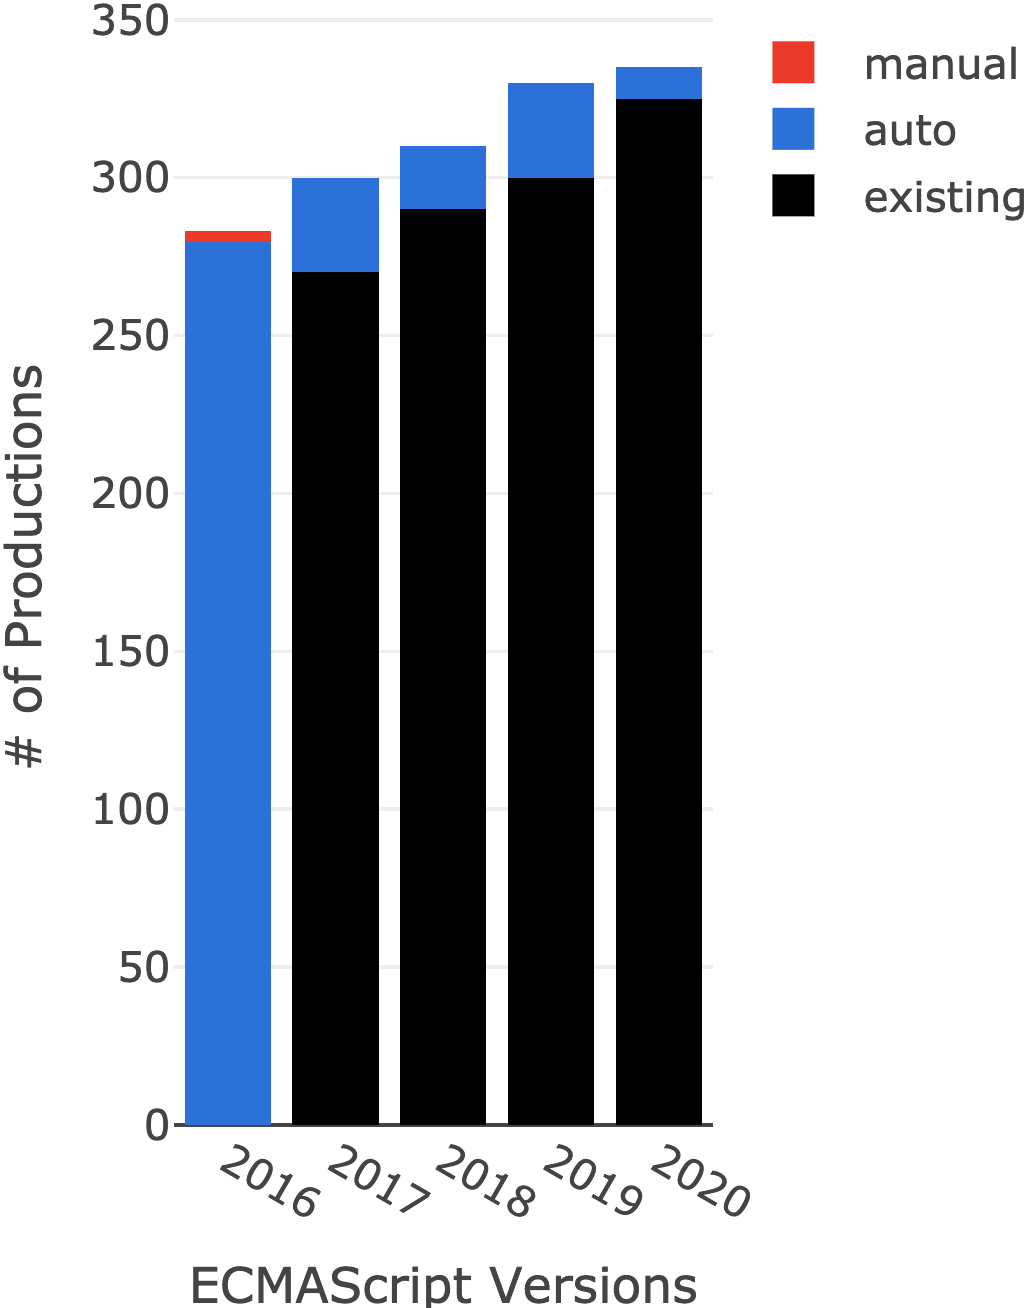
\includegraphics[width=\textwidth]{img/all-version-syntax.png}
    \caption{The parser generator.}
    \label{fig:syntax-all-version}
  \end{subfigure}
  \hfill
  \begin{subfigure}{0.23\textwidth}
    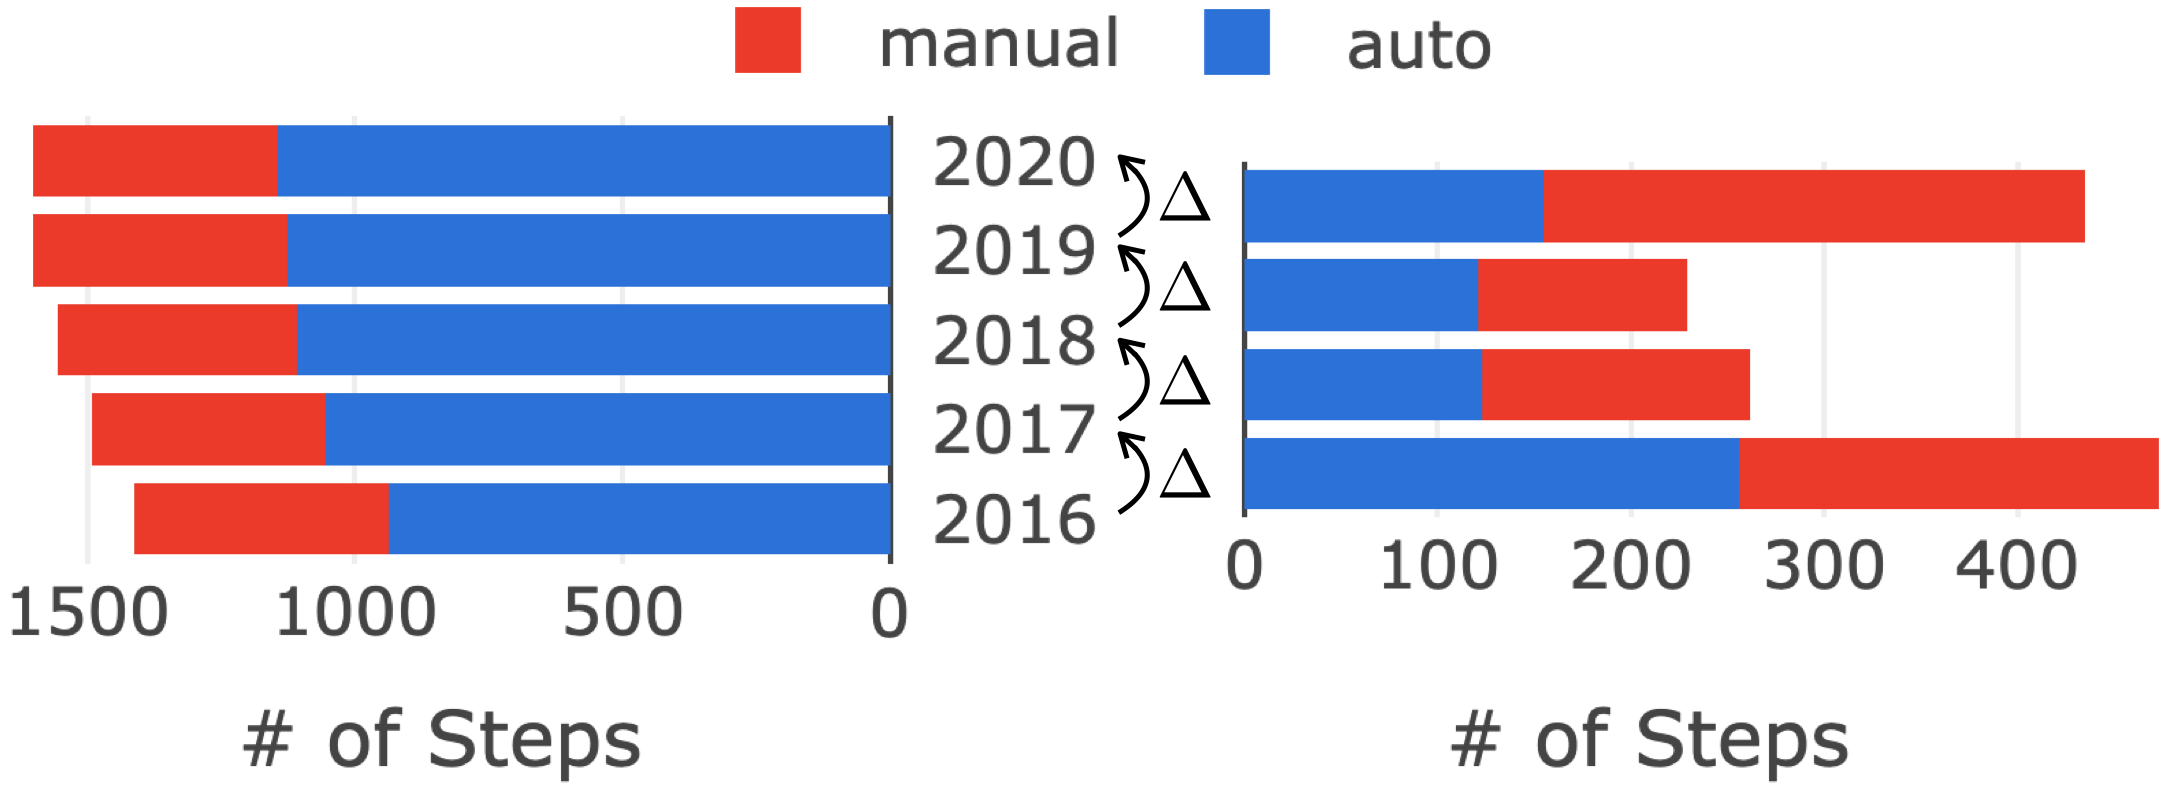
\includegraphics[width=\textwidth]{img/all-version-sem.png}
    \caption{The algorithm compiler.}
    \label{fig:semantics-all-version}
  \end{subfigure}
  \caption{The result of the parser generator and the algorithm compiler for
  ECMAScript specifications from 2016 to 2020.}
  \label{fig:all-version}
\end{figure}

We discuss the effectiveness of \( \tool \) by applying it into existing ECMAScript specifications.
The evaluation focuses on how many productions and abstract algorithms are covered by
our tool 1) in each version, and 2) in each difference between adjacent versions.
Figure~\ref{fig:all-version} shows the result of \( \tool \) from ECMAScript 2016
to 2020. While ECMAScript 5.1 is the first version that officially supports
the specification in HTML. However, two oldest versions ECMAScript 5.1 and 2015 are written
in quite different styles with recent versions including HTML tags used in abstract algorithms.
Thus, we evaluate only five recent versions from ECMAScript 2016 to 2020.
As described in Figure~\ref{fig:all-version}, \( \tool \) suceeds to generate parsers
from all versions. For semantics, the algorithm compiler has \inred{XX\%} success rates
in average. Moreover, \( \tool \) are also effective to update existing semantics
because \inred{XX\%} of newly defined algorithms are automatically compiled into \( \ires \)
functions.

\subsection{Correctness}

\begin{table}
  \centering
  \begin{tabular}{lr}\toprule
    \belowrulesepcolor{gainsboro}
    \rowcolor{gainsboro} \textbf{All tests262 Tests} & \textbf{36,794} \\
    \aboverulesepcolor{gainsboro}\midrule
    Annexes/Internationalisation & 1,774\\ \hdashline
    In-process features & \inred{XXXX} \\\hdashline
    Module tests & \inred{XXXX} \\\hdashline
    Non-strict tests & \inred{XXXX} \\\midrule
    \belowrulesepcolor{gainsboro}
    \rowcolor{gainsboro} \textbf{ECMAScript 2020 Strict Script Tests} & \textbf{\inred{XXXXX}} \\
    \aboverulesepcolor{gainsboro}\midrule
    Not supported features & \inred{XXXX} \\\midrule
    \belowrulesepcolor{gainsboro}
    \rowcolor{gainsboro} \textbf{Applicable Tests} & \textbf{\inred{XXXXX}} \\
    \aboverulesepcolor{gainsboro}\midrule
    Passed tests & \inred{XXXX} \\\hdashline
    Failed tests & \inred{XXXX} \\\bottomrule
  \end{tabular}
  \caption{The results of tests in the test262 for ECMAScript 2020.}
  \label{table:test262}
\end{table}

To evaluate that \( \tool \) correctly extracts semantics, we extract semantics of ECMAScript
2020 via our tool. Above automatically extracted parts of semantics, we manually implement
\inred{XX} \( \ires \) functions for failed to be automatically compiled abstract algorithms.
Moreover, we fill in global setting based on ECMAScript 2020 specification as described
in Section~\ref{sec:framework}. The ECMAScript 2020 version is actively updated in
GitHub~\ref{es2020} to be released in the next year. Ecma Technical Committee 39 (TC39)
officially provides the conformance test suite, test262, for ECMAScript 2020.
Thus, we decide to evaluate the correctness of our syntax and semantics based on the test262.
However, the test262 also provides tests for in-process features and other extensions
such as web browsers and internationalisation. Thus, we exclude them from our target tests.
Figure~\ref{table:test262} describes how to break down tests and the test results of extracted
semantics. We use test262 written in \inred{August 6, 2019}. In that version,
test262 consists of 36,794 tests and we first exclude \inred{XXXX} tests
for extensions and in-process features. Then, we remove tests for non-strict mode because
we focus on only JavaScript codes in strict mode
as described in Section~\ref{sec:framework}. Finally, we remove the \inred{XXXX} tests
for not supported language features such as \inred{modules, JSON, RegExp, or Date}.
We test our extracted semantics for \inred{XXXXX} applicable tests and pass \inred{XXXX} tests.
There are several reasons of test failures; \inred{...}.

\subsection{Adaptability}

\begin{table}
  \centering
  \[
    \begin{array}{l|r|r|r|r} \hline
      \text{features} &
      \multicolumn{1}{c|}{\text{\#prods}} &
      \multicolumn{1}{c|}{\text{\#steps}} &
      \multicolumn{1}{c|}{\Delta\text{CR}} &
      \multicolumn{1}{c}{\text{tests}}\\\hline
      \text{\inred{????}} & \inred{X} & \inred{XX} & \inred{X} & \inred{XX/XX}\\\hline
      \text{\inred{????}} & \inred{X} & \inred{XX} & \inred{X} & \inred{XX/XX}\\\hline
      \text{\inred{????}} & \inred{X} & \inred{XX} & \inred{X} & \inred{XX/XX}\\\hline
      \text{\inred{????}} & \inred{X} & \inred{XX} & \inred{X} & \inred{XX/XX}\\\hline
      \text{\inred{????}} & \inred{X} & \inred{XX} & \inred{X} & \inred{XX/XX}\\\hline
      \text{\inred{????}} & \inred{X} & \inred{XX} & \inred{X} & \inred{XX/XX}\\\hline
      \text{\inred{????}} & \inred{X} & \inred{XX} & \inred{X} & \inred{XX/XX}\\\hline
      \text{\inred{????}} & \inred{X} & \inred{XX} & \inred{X} & \inred{XX/XX}\\\hline
      \text{\inred{????}} & \inred{X} & \inred{XX} & \inred{X} & \inred{XX/XX}\\\hline
      \text{\inred{????}} & \inred{X} & \inred{XX} & \inred{X} & \inred{XX/XX}\\\hline
      \text{\inred{????}} & \inred{X} & \inred{XX} & \inred{X} & \inred{XX/XX}\\\hline
      \text{\inred{????}} & \inred{X} & \inred{XX} & \inred{X} & \inred{XX/XX}\\\hline
      \text{\inred{????}} & \inred{X} & \inred{XX} & \inred{X} & \inred{XX/XX}\\\hline
      \hline
      \text{total} & \inred{XX} & \inred{XXX} & \inred{XX} & \inred{XXX/XXX}\\\hline
    \end{array}
  \]
  \caption{The result of \( \tool \) for in-process language features}
  \label{table:in-process}
\end{table}

We also check that \( \tool \) deals with future language features for adaptability.
ECMAScript specifications are managed as open-sources and proposals of in-process language
features follow the TC39 process and are tracked in the separated repository~\ref{proposals}.
Thare are five stages for proposals; Stage 0, Stage 1, active, finished or inactive proposals.
Each proposal starts from Stage 0 and is promoted to an active proposal through Stage 1.
Then, the committee (TC39) regularly examins the active proposal and changes the stage into
finished if they want to apply the proposed language features, otherwise, changes it
into inactive stage.



% We also check that \( \tool \) deals with future language features based on in-process language
% features. Each in-process language feature has its own specification, and the test262 supports
% tests for them. We extract semantics of \inred{XX} language features via \( \tool \) and test extracted
% semantics based on tests in test262. Table~\ref{table:in-process} describes the result and
% \( \tool \) successfully generates parsers of total \inred{XX} productions.
% For semantics, \( \tool \) successfully compiles \inred{XXX} algorithm steps by adding
% \inred{XX} more compile rules. Above the semantics, \inred{XXX} tests passes among \inred{XXX}
% tests for \inred{XX} in-process language features.


\subsection{Specification Error Detection}

We found four specification errors in ECMAScript 2020. All of them 



% test262 결과를 어떻게? 전체 개수 / applicable tests 개수 / succes, fail 개수
% \inred{refactoring for compile rules / get statistics of compile rules}
% 개수만 - stmt / expr / cond / ref 몇개씩? / corner cases 개수
% \inred{proposed language features / related tests in test262 / diff of compile rules}
% 각 feature name / 의미 / compile 성공률 / 결과 test
% \inred{supprot "Assert: ... "?/ confirm found spec errors by TC39}
